\chapter{工具应用效果的多因素分析方法研究}
\label{chap:r46-4}

本项研究整理12口井2040条现场日报记录及三类套磨铣工具的四组360个室内实验工况，构建由现场作业和室内实验两部分组成的工具应用数据集。按工具类型、工件材料及作业参数开展分组分析，研究钻压、转速与钻速、扭矩和磨损量之间的关系，并通过Power BI提供记录和照片查询。

在钻压$2\sim20$ kN、转速$20\sim100$ r/min的室内实验范围内，钻压是影响钻速变化的主要作业参数，转速的作用随钻压区间增强。不同工具类型与工件材料对应的提速、扭矩和磨损关系存在差异，为分别建立性能预测模型和优选作业参数提供了依据。

\section{现场作业与室内实验数据集构建}
\label{sec:r46-4.1}

数据集由现场作业和室内实验两部分组成。现场数据保留井号、工艺类型、记录中提及的工具、作业趟次、处理对象、参数变化、进尺及出井检查；室内数据按实验工具、工件材料、钻压和转速整理钻速、扭矩及磨损量。工具名称和规格等信息以现场记录及实验记录中的记载为依据，主要内容见表4-1。

\begin{table}[H]
\centering
\setstretch{1}
\fontsize{12}{15}\selectfont
\setlength{\tabcolsep}{3pt}
\renewcommand{\arraystretch}{1.5}
\caption{工具应用数据集的主要内容}\label{tab:r46-4-1}
\begin{tabular}{>{\centering\arraybackslash}m{0.204792\dimexpr\linewidth-6\tabcolsep-4\arrayrulewidth\relax}>{\centering\arraybackslash}m{0.433422\dimexpr\linewidth-6\tabcolsep-4\arrayrulewidth\relax}>{\centering\arraybackslash}m{0.361787\dimexpr\linewidth-6\tabcolsep-4\arrayrulewidth\relax}}
\toprule
 资料类别 & 记录内容 & 已形成的数据 \\ \midrule
现场作业 & 井号、工艺类型、记录中的工具信息、趟次、参数变化、进尺及出井检查 & 12口井、2040条原始记录；47组连续作业 \\ 
室内套磨铣实验 & 实验工具、工件材料、钻压、转速及三项性能 & 三类工具、两种材料；四组360个工况、1080项数值 \\ \bottomrule
\end{tabular}
\end{table}

现场记录按井号、工具趟次及连续作业过程归组，保留原始文字、所在工作表和相关照片，便于核对参数调整与作业效果。室内记录按三类工具和两种工件材料分为四组，每组90个工况，每个工况对应钻速、扭矩和磨损量三项性能值，共360个工况、1080项数值。

\section{现场日报整理与作业过程分析}
\label{sec:r46-4.2}

\subsection{现场数据整理}
\label{sec:r46-4.2.1}

现场数据来自12口井的日报，共整理362张日报工作表中的2040条原始作业记录。按同井、同趟工具和同一次连续作业归并，保留调参、推进、循环及检查的先后关系，形成47组连续作业。各类别的数据量见表4-2。

\begin{table}[H]
\centering
\setstretch{1}
\fontsize{12}{15}\selectfont
\setlength{\tabcolsep}{3pt}
\renewcommand{\arraystretch}{1.5}
\caption{现场日报的分析数据量}\label{tab:r46-4-2}
\begin{tabular}{>{\centering\arraybackslash}m{0.200000\dimexpr\linewidth-10\tabcolsep-6\arrayrulewidth\relax}>{\centering\arraybackslash}m{0.200000\dimexpr\linewidth-10\tabcolsep-6\arrayrulewidth\relax}>{\centering\arraybackslash}m{0.200000\dimexpr\linewidth-10\tabcolsep-6\arrayrulewidth\relax}>{\centering\arraybackslash}m{0.200000\dimexpr\linewidth-10\tabcolsep-6\arrayrulewidth\relax}>{\centering\arraybackslash}m{0.200000\dimexpr\linewidth-10\tabcolsep-6\arrayrulewidth\relax}}
\toprule
 作业类型 & 涉及井数 & 工具趟次 & 连续作业组 & 参数及过程阶段数 \\ \midrule
磨铣 & 4 & 5 & 5 & 9 \\ 
套铣 & 7 & 14 & 19 & 64 \\ 
切割 & 7 & 19 & 23 & 79 \\ 
合计 & 12口井 & 按作业类型统计 & 47 & 152 \\ \bottomrule
\end{tabular}
\end{table}

切割作业以水力切割为主，23组作业中包括18次水力切割、4次电动机械切割和1次镁基切割。按各次作业的参数调整过程划分阶段，可对照分析参数变化前后的作业情况。

磨铣和套铣资料中，整理得到66条作业参数与工作扭矩配对记录，以及49个作业参数与进尺能够对应的记录时段，为参数对照和作业过程分析提供了基础。

\subsection{作业参数与效果的现场对照}
\label{sec:r46-4.2.2}

套铣资料中有7个作业组可计算参数与扭矩的相关系数，其中4组至少包含6个参数阶段。钻压和扭矩按日报所记范围的中点计算Spearman秩相关。为检查少量记录对结果的影响，依次暂不计入其中一条日报记录，用其余记录重新计算相关系数；将各次计算得到的最小值和最大值列为“相关系数复算范围”。典型结果见表4-3。

\begin{table}[H]
\centering
\setstretch{1}
\fontsize{12}{15}\selectfont
\setlength{\tabcolsep}{3pt}
\renewcommand{\arraystretch}{1.5}
\caption{典型套铣作业中钻压与地面扭矩的相关性}\label{tab:r46-4-3}
\begin{tabular}{>{\centering\arraybackslash}m{0.250000\dimexpr\linewidth-8\tabcolsep-5\arrayrulewidth\relax}>{\centering\arraybackslash}m{0.250000\dimexpr\linewidth-8\tabcolsep-5\arrayrulewidth\relax}>{\centering\arraybackslash}m{0.250000\dimexpr\linewidth-8\tabcolsep-5\arrayrulewidth\relax}>{\centering\arraybackslash}m{0.250000\dimexpr\linewidth-8\tabcolsep-5\arrayrulewidth\relax}}
\toprule
 连续作业组 & 参数阶段数 & 相关系数ρ & 相关系数复算范围 \\ \midrule
BZ34-9-A26 第1趟第1组 & 9 & −0.834 & $-0.929\sim-0.761$ \\ 
BZ34-9-A26 第4趟第1组 & 12 & −0.476 & $-0.658\sim-0.306$ \\ 
CFD6-4-A5 第2趟第2组 & 6 & +0.277 & $-0.224\sim+0.860$ \\ 
SZ36-1-A21 第1趟第1组 & 6 & +1.000 & $+1.000\sim+1.000$ \\ \bottomrule
\end{tabular}
\end{table}

BZ34-9-A26的两组结果呈负相关，SZ36-1-A21组呈正相关；CFD6-4-A5组在复算中出现相关系数正负转换，说明相关判断容易受到少量记录的影响。同一参数在不同作业组中的变化关系存在差异，需要结合具体井况和作业过程分析。

日报记录了参数变化与进尺变化不同步的现象。A26第4趟套铣将转速从$30\sim40$ r/min提高到$60\sim70$ r/min后，地面扭矩升高，后续两个时段仍没有新增进尺。WZ11-1-A11S1第1趟磨铣的两段工作扭矩均为$5.63\sim7.46$ kN·m，前段19.5 h内进尺0.52 m，后段2.5 h无进尺。现场效果评价需要结合扭矩与进尺的变化共同判断。

在A26第3趟套铣中，活动管柱、替入5 m³稠塞并调整参数后，累计进尺由0.10 m增加到0.15 m，反映出联合处理后的作业改善。A26第1趟后期则出现钻压增大、进尺逐渐减慢的情况。这些过程记录显示，现场参数调整往往伴随井下作业条件变化。

切割资料中，11次具有初始阶段起止扭矩记录的作业有10次扭矩中点下降；10次可比较末段与同转速空转扭矩的作业中，有8次报告范围重叠。这些现象可辅助观察切割过程，但切断结果仍需结合提活、割口或打捞记录确认。LD5-2N-A19的C02作业在排量降回10 m³/h后，泵压仍为8.3 MPa，高于同排量早期的$1.82\sim2.84$ MPa；出井试验发现马达不能正常旋转，说明压力升高还可能与设备异常有关。

\subsection{现场应用效果的评价方法}
\label{sec:r46-4.2.3}

现场分析按同趟工具和处理对象比较参数变化，结合起下钻、活动管柱、循环及出井检查解释作业响应。地面扭矩包含工具工作负载与管柱摩阻；采用井下马达时，地面转速与刀具实际转速分别记录。井况、工具组合和辅助处置作为同组比较的条件保留，避免把不同作业过程合并为统一的钻压—扭矩关系。

现场推进率按对应日报时段的新增进尺与过程时间计算，用于评价该时段的作业进展。室内钻速按工件钻除深度与实际钻除时间计算。现场累计时间中的起下钻、循环和检查分别保留，室内钻速使用实际钻除时间。

现场资料用于识别调参、停滞、恢复推进和工具异常等过程特征；室内参数网格用于比较相同工具、材料条件下的钻压与转速响应。两类分析相互补充：现场记录解释工况差异，室内数据提供可对照的性能关系。

\section{室内套磨铣实验及分析方法}
\label{sec:r46-4.3}

\subsection{实验装置与工具材料}
\label{sec:r46-4.3.1}

室内套磨铣实验采用油气井筒清洁工具工作性能实验系统。装置包括工具与工件夹持机构、旋转驱动模块、钻压控制模块和信号采集显示模块，配备超景深显微成像系统、电子天平等测量设备。装置与装夹形式见图4-1。

\begin{figure}[H]
\centering
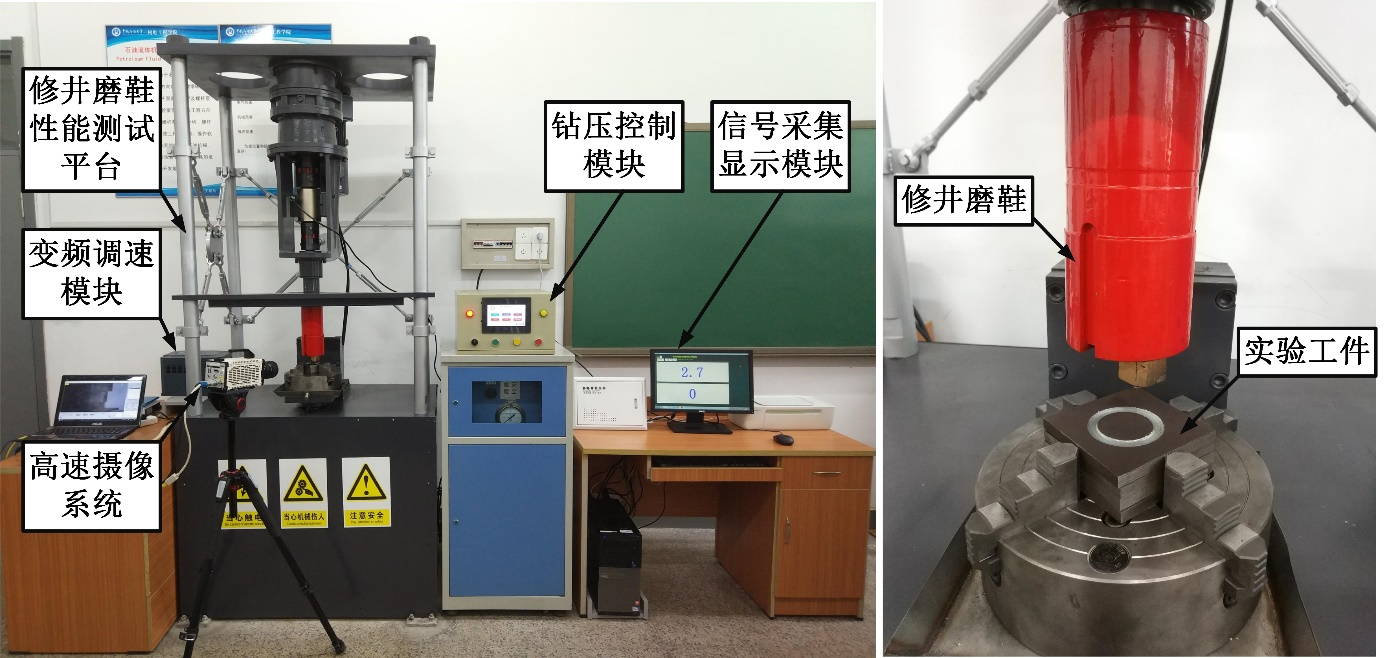
\includegraphics[width=145.000mm,height=0.76\textheight,keepaspectratio]{figure/research4-6/fig4-01-1.jpg}
\caption{套磨铣实验系统及工具工件装夹}
\label{fig:r46-4-1}
\end{figure}

装置的转速调节范围为$20\sim200$ r/min，轴向加载范围为$0\sim20$ kN。本次实验选取钻压$2\sim20$ kN、转速$20\sim100$ r/min进行分析。工装适配工具外径$100\sim110$ mm、含堆焊磨粒总长$230\sim240$ mm及NC26母扣连接。采用平底式磨铣、刀翼式磨铣和套铣三类工具，与45号钢、铸铁形成表4-4所列的四组实验条件。

\begin{table}[H]
\centering
\setstretch{1}
\fontsize{12}{15}\selectfont
\setlength{\tabcolsep}{3pt}
\renewcommand{\arraystretch}{1.5}
\caption{室内套磨铣实验的工具与材料}\label{tab:r46-4-4}
\begin{tabular}{>{\centering\arraybackslash}m{0.250000\dimexpr\linewidth-8\tabcolsep-5\arrayrulewidth\relax}>{\centering\arraybackslash}m{0.250000\dimexpr\linewidth-8\tabcolsep-5\arrayrulewidth\relax}>{\centering\arraybackslash}m{0.250000\dimexpr\linewidth-8\tabcolsep-5\arrayrulewidth\relax}>{\centering\arraybackslash}m{0.250000\dimexpr\linewidth-8\tabcolsep-5\arrayrulewidth\relax}}
\toprule
 实验分组 & 工具 & 工件材料 & 钻压与转速组合数 \\ \midrule
第1组 & 平底式磨铣工具 & 45号钢 & 90 \\ 
第2组 & 刀翼式磨铣工具 & 45号钢 & 90 \\ 
第3组 & 套铣工具 & 45号钢 & 90 \\ 
第4组 & 套铣工具 & 铸铁 & 90 \\ \bottomrule
\end{tabular}
\end{table}

\subsection{实验参数与性能指标}
\label{sec:r46-4.3.2}

每组设置10个钻压水平（$2\sim20$ kN，间隔2 kN）和9个转速水平（$20\sim100$ r/min，间隔10 r/min），形成90个参数组合。四组共360个工况，对应钻速、工作扭矩和磨损量1080项指标值。三项指标按相同工具、材料、钻压和转速配对，原始矩阵保留于分析测试（实验）报告附录。

钻速由工件钻除深度与钻除时间计算，工作扭矩由信号采集模块获取，磨损量为试前与试后工具质量差，单位为g。磨损量用于比较各工况的工具消耗；耐用性评价另按累计运行时间、行程或循环次数及功能保持情况记录。

\subsection{多因素分析方法}
\label{sec:r46-4.3.3}

按工具与材料分组，计算钻压、转速、钻速、扭矩和磨损量的Pearson相关系数。以钻速总平方和为基准，比较钻压和转速各水平均值对应的变异占比，描述本参数网格中的主要响应。再按$2\sim10$ kN、$12\sim16$ kN和$18\sim20$ kN划分钻压区间，识别各区间内转速作用的变化。

在相同钻压、转速下，以平底式和刀翼式磨铣工具加工45号钢的实验结果比较工具类型的影响，以同一套铣工具加工45号钢和铸铁的结果比较工件材料的影响。第五章在此基础上综合考虑钻速、扭矩和磨损量，开展多目标作业参数优选。

\section{室内实验的影响因素分析结果}
\label{sec:r46-4.4}

\subsection{钻压与各项性能的关系}
\label{sec:r46-4.4.1}

四组实验中，钻压与钻速的相关系数为$0.772\sim0.949$，与扭矩为$0.361\sim0.905$，与磨损量为$0.781\sim0.991$，均高于对应转速与性能的整体相关系数。两类磨铣工具中，钻压与磨损量的相关系数分别为0.987和0.991，提高钻压时，钻速增加通常伴随工具磨损增加。图4-2的上三角为相关系数，下三角为散点与线性趋势，对角线为各参数的数据分布。

\begin{figure}[H]
\centering
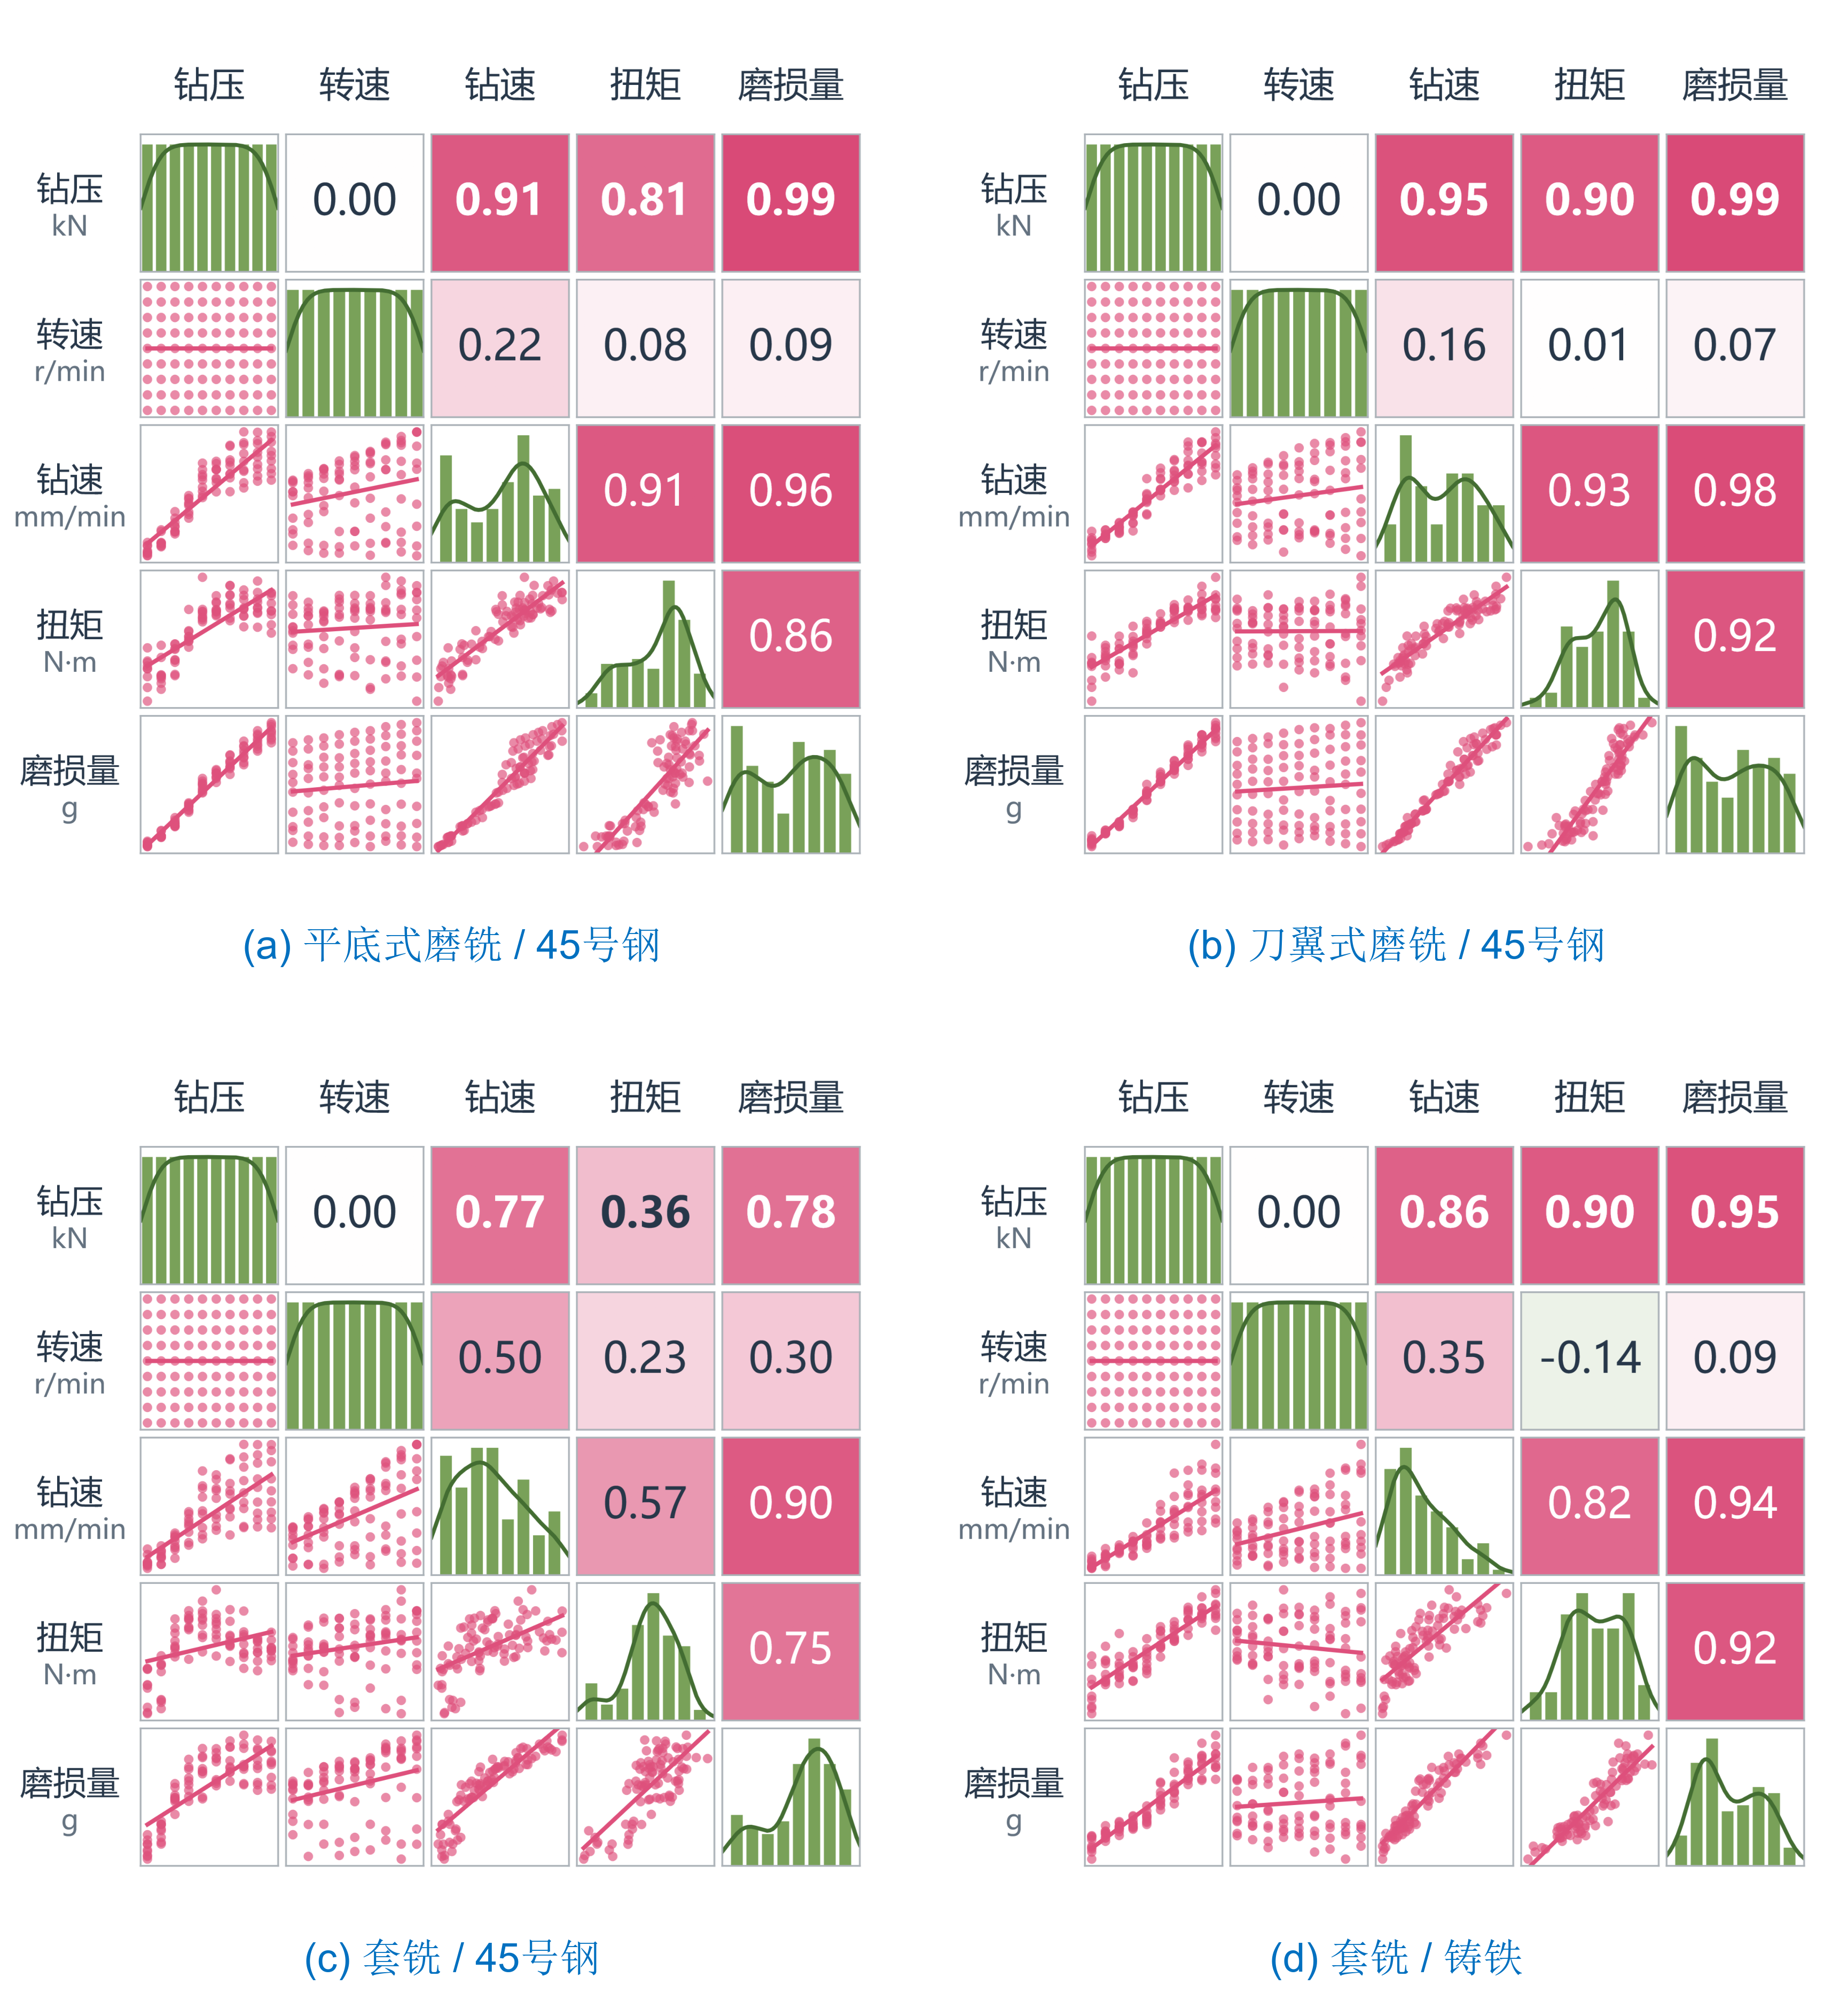
\includegraphics[width=145.000mm,height=0.76\textheight,keepaspectratio]{figure/research4-6/fig4-02-1.png}
\caption{四组工具与材料条件下的五变量相关性矩阵}
\label{fig:r46-4-2}
\end{figure}

对钻速变化进行分解，四组中由钻压水平差异解释的变异占比分别为89.5\%、91.8\%、64.7\%和75.4\%，由转速水平差异解释的占比分别为5.1\%、2.9\%、25.3\%和12.3\%。结合相关系数与曲线比较，钻压是本次实验范围内与钻速变化关系较强的因素，转速的作用在套铣组中比两类磨铣组更明显。

在高钻压区间，继续加压的收益因工具和材料而异。按同一钻压下9个转速的结果等权平均，钻压由16增至20 kN时，平底式磨铣平均钻速由9.19增至9.58 mm/min，提高4.3\%，平均磨损量由4.44增至5.21 g，提高17.5\%；套铣45号钢的平均钻速由13.15增至13.45 mm/min，提高2.2\%，平均扭矩和磨损量分别降低2.9\%和1.8\%。同一区间内，刀翼式磨铣和套铣铸铁平均钻速分别提高10.7\%和17.6\%，平均磨损量分别增加20.3\%和16.0\%。选参时需分别比较各组的提速、负载和磨损变化。图4-3以散点展示各转速下的实测值，连线表示同一钻压下的平均钻速，标注数值为$16\sim20$ kN区间的平均钻速增幅。

\begin{figure}[H]
\centering
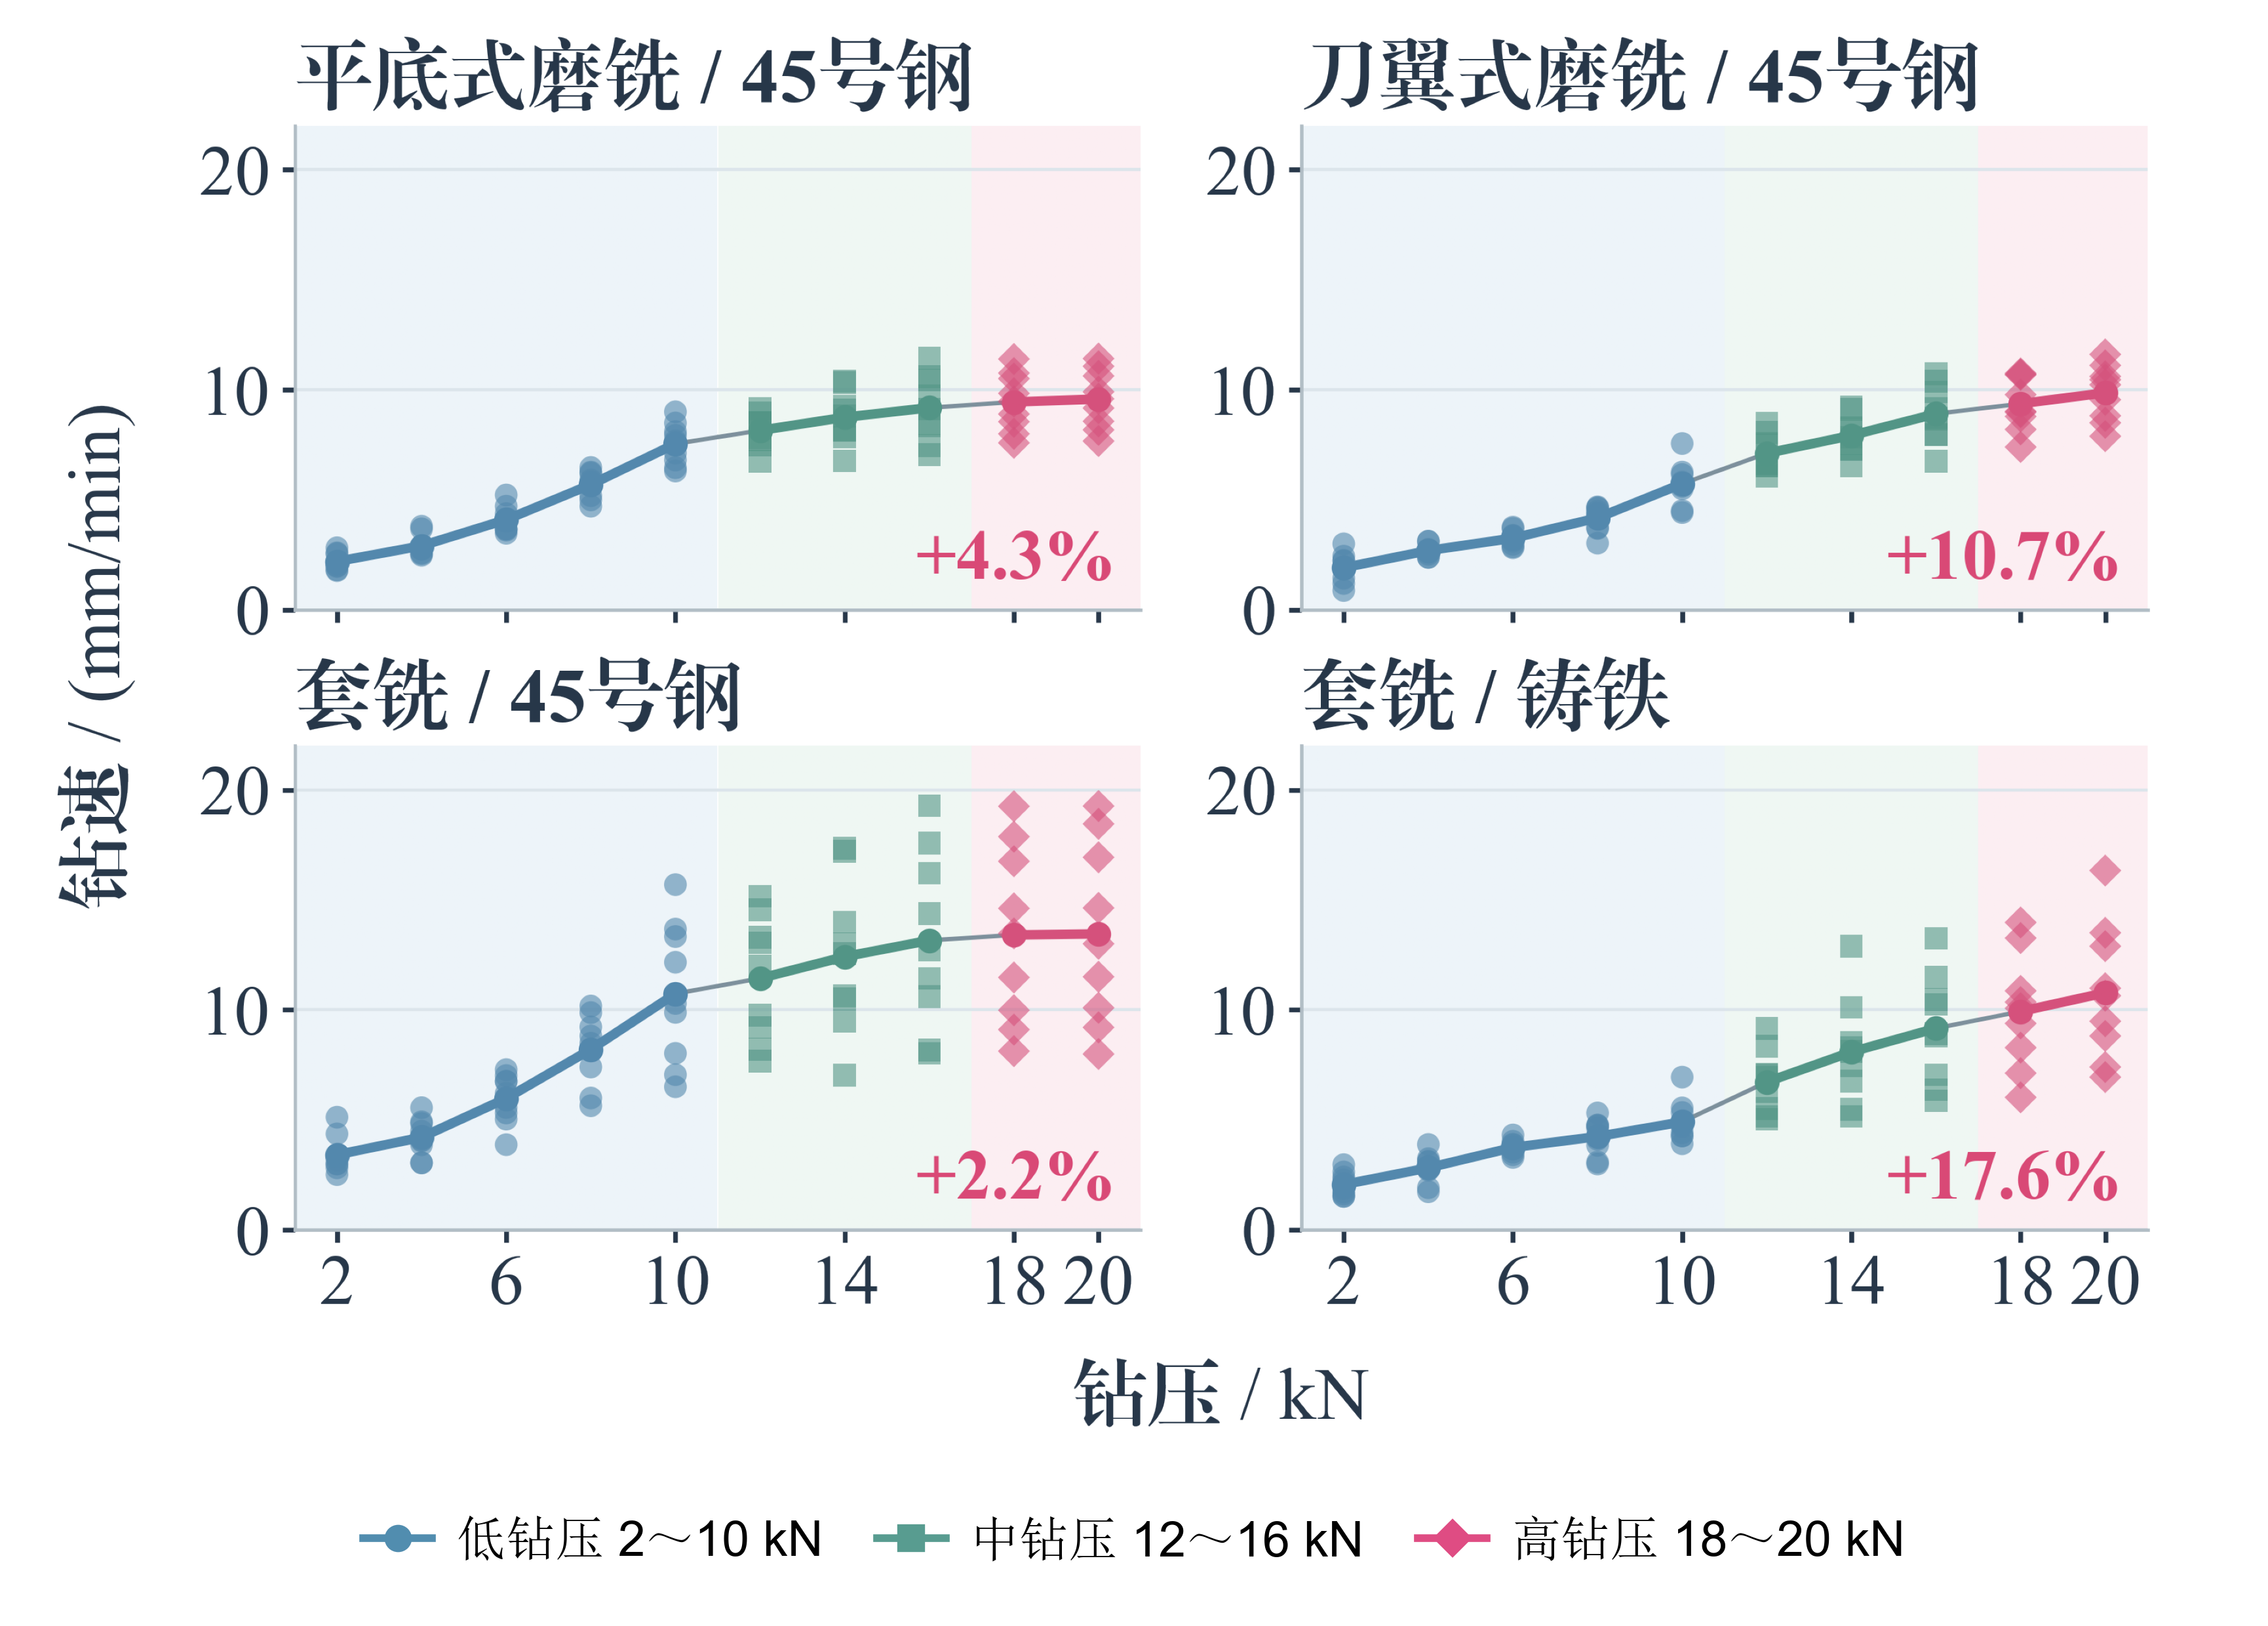
\includegraphics[width=145.000mm,height=0.76\textheight,keepaspectratio]{figure/research4-6/fig4-03-1.png}
\caption{四组实验中钻速随钻压的变化}
\label{fig:r46-4-3}
\end{figure}

\subsection{转速与性能的关系随钻压区间变化}
\label{sec:r46-4.4.2}

整个实验范围内，转速与钻速的相关系数为$0.163\sim0.502$，低于钻压与钻速的相关系数；转速与扭矩、磨损量的相关性也较弱。按钻压分区后，各项关系明显变化，见图4-4。低、中、高钻压区间分别为$2\sim10$ kN、$12\sim16$ kN和$18\sim20$ kN。

\begin{figure}[H]
\centering
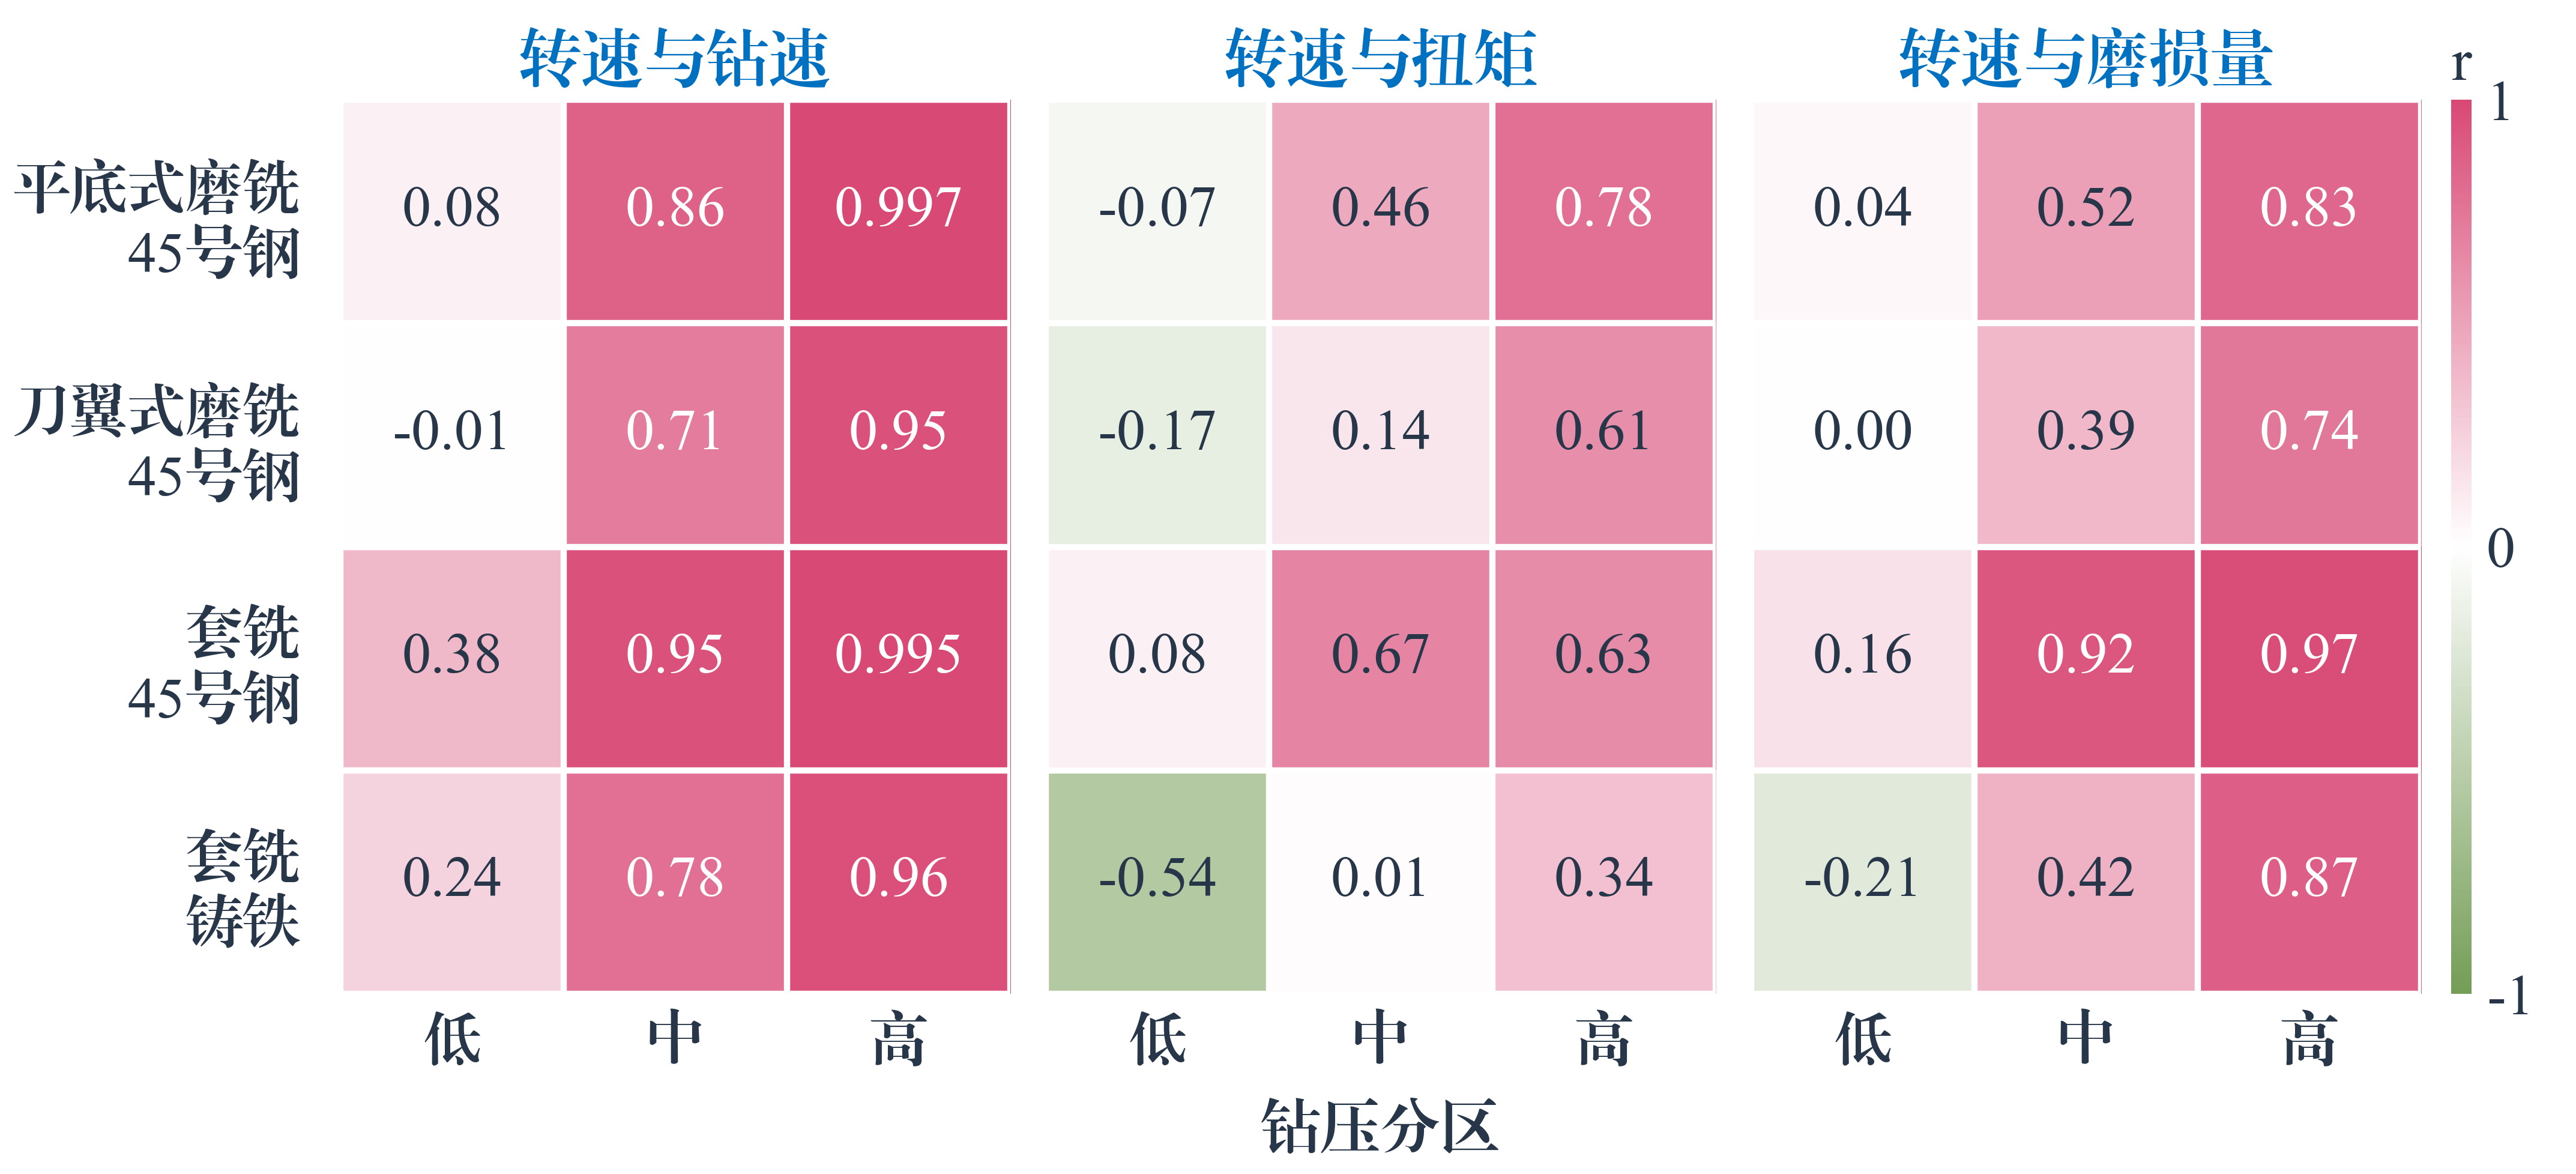
\includegraphics[width=145.000mm,height=0.76\textheight,keepaspectratio]{figure/research4-6/fig4-04-1.png}
\caption{不同钻压区间内转速与三项性能的相关性}
\label{fig:r46-4-4}
\end{figure}

低、中、高钻压区间内，转速与钻速的相关系数分别为$-0.005\sim0.379$、$0.705\sim0.951$和$0.953\sim0.997$。固定16 kN，将转速由20提高至100 r/min时，四组钻速分别由7.47、6.76、8.02和5.87 mm/min提高到11.43、10.73、19.28和13.24 mm/min，显示提高转速的收益与钻压条件相互配合。

分区结果还表明，在高钻压区间，转速与扭矩的相关系数为$0.34\sim0.78$，与磨损量为$0.74\sim0.97$。提高转速带来提速效果的同时，负载与磨损也会发生变化，需要结合具体工具和材料综合选参。

\subsection{工具类型与工件材料的影响}
\label{sec:r46-4.4.3}

\begin{table}[H]
\centering
\setstretch{1}
\fontsize{12}{15}\selectfont
\setlength{\tabcolsep}{3pt}
\renewcommand{\arraystretch}{1.5}
\caption{四组实验的实测性能范围}\label{tab:r46-4-5}
\begin{tabular}{>{\centering\arraybackslash}m{0.250000\dimexpr\linewidth-8\tabcolsep-5\arrayrulewidth\relax}>{\centering\arraybackslash}m{0.250000\dimexpr\linewidth-8\tabcolsep-5\arrayrulewidth\relax}>{\centering\arraybackslash}m{0.250000\dimexpr\linewidth-8\tabcolsep-5\arrayrulewidth\relax}>{\centering\arraybackslash}m{0.250000\dimexpr\linewidth-8\tabcolsep-5\arrayrulewidth\relax}}
\toprule
 工具与材料 & 钻速\newline{}(mm/min) & 扭矩\newline{}(N·m) & 磨损量\newline{}(g) \\ \midrule
平底式磨铣45号钢 & $1.78\sim11.43$ & $12.21\sim36.64$ & $0.96\sim5.58$ \\ 
刀翼式磨铣45号钢 & $0.88\sim11.61$ & $7.39\sim39.52$ & $0.78\sim5.62$ \\ 
套铣45号钢 & $2.51\sim19.28$ & $32.23\sim70.53$ & $1.98\sim8.50$ \\ 
套铣铸铁 & $1.52\sim16.33$ & $17.03\sim78.88$ & $0.68\sim11.99$ \\ \bottomrule
\end{tabular}
\end{table}

在加工45号钢的90个相同钻压、转速工况中，刀翼式磨铣相对平底式磨铣的平均钻速、扭矩和磨损量分别变化−9.8\%、−4.2\%和−4.1\%。刀翼式磨铣在20 kN、100 r/min时取得11.61 mm/min的单点最高钻速。比较两类工具时，应同时考虑整个实验参数范围内的钻速、扭矩和工具消耗。

同一套铣工具加工铸铁时，相对加工45号钢的平均钻速低35.2\%，平均扭矩低4.8\%，平均磨损量低0.6\%；而在16、18、20 kN的27组相同参数设置下，铸铁组的平均扭矩和磨损量分别高27.1\%和33.0\%。材料变化不仅影响平均性能，还改变高载荷区间的扭矩和磨损水平。两类套铣材料条件因此需要分别分析和建模。

同一工具、材料条件下，提高钻速常伴随扭矩和磨损变化。不同工具类型及工件材料分别分析，作业参数优选据此综合考虑效率要求、工作负载与工具消耗。

\section{应用数据集与可视化查询}
\label{sec:r46-4.5}

井筒工具应用数据集设置“现场数据”和“室内实验数据”两个页面。现场页面按井号、工艺类型及工具查询作业过程，室内页面按工具、工件材料和实验参数查询性能结果，并关联相应照片。

\subsection{现场数据查询}
\label{sec:r46-4.5.1}

现场页面覆盖12口井，关联136张照片。选择井号、工艺类型、工具名称及趟次后，可查看参数变化、进尺与出井检查。磨铣、套铣记录显示钻压及地面扭矩，切割记录显示排量及泵压，并可回查作业原文。

\begin{figure}[H]
\centering
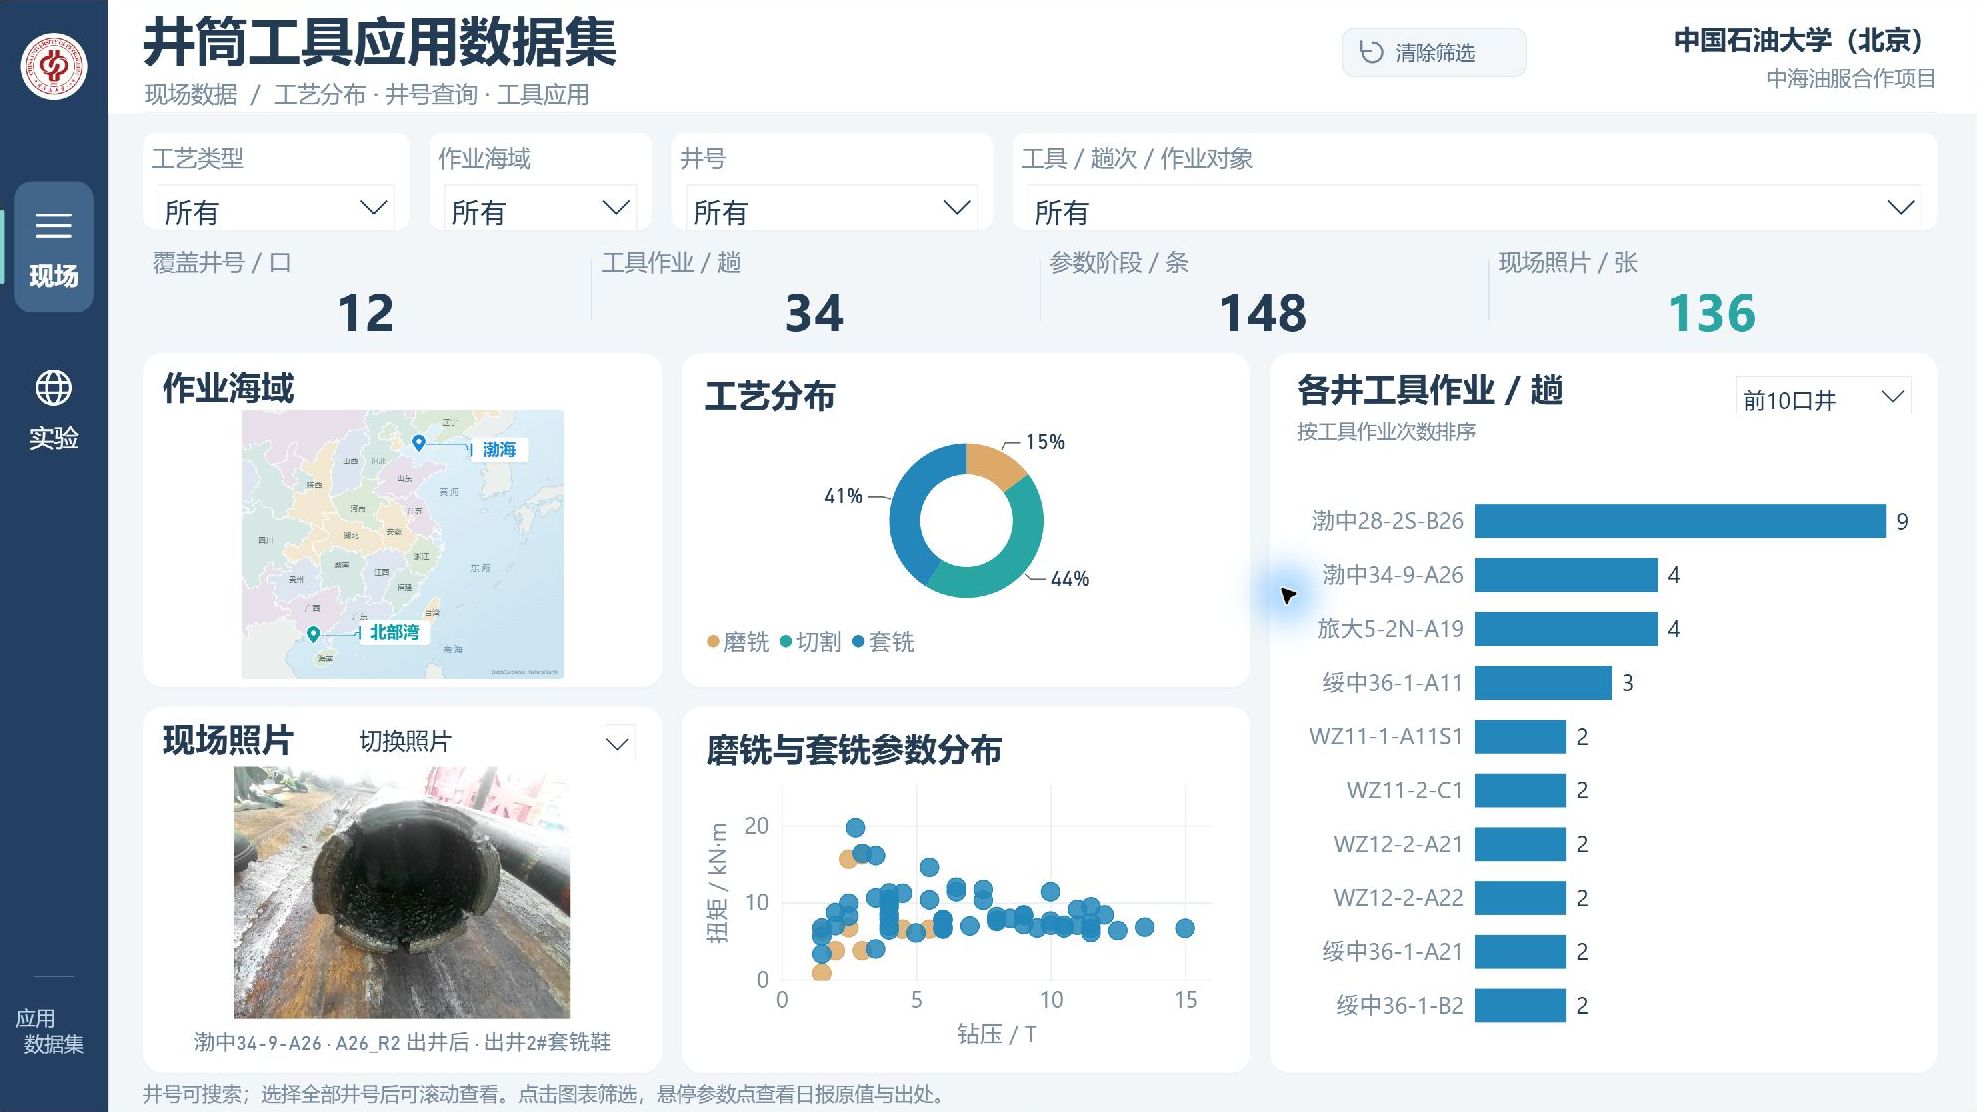
\includegraphics[width=120.000mm,height=0.76\textheight,keepaspectratio]{figure/research4-6/fig4-05-1.png}
\caption{井筒工具应用数据集现场查询界面}
\label{fig:r46-4-5}
\end{figure}

\subsection{室内实验查询与数据维护}
\label{sec:r46-4.5.2}

室内页面收录四组360个工况，可按工具、材料、钻压和转速查询钻速、扭矩及质量损失。参数矩阵显示钻速随钻压、转速的分布，散点图用于对照效率与负载，照片关联到工具、装夹和测量过程。

\begin{figure}[H]
\centering
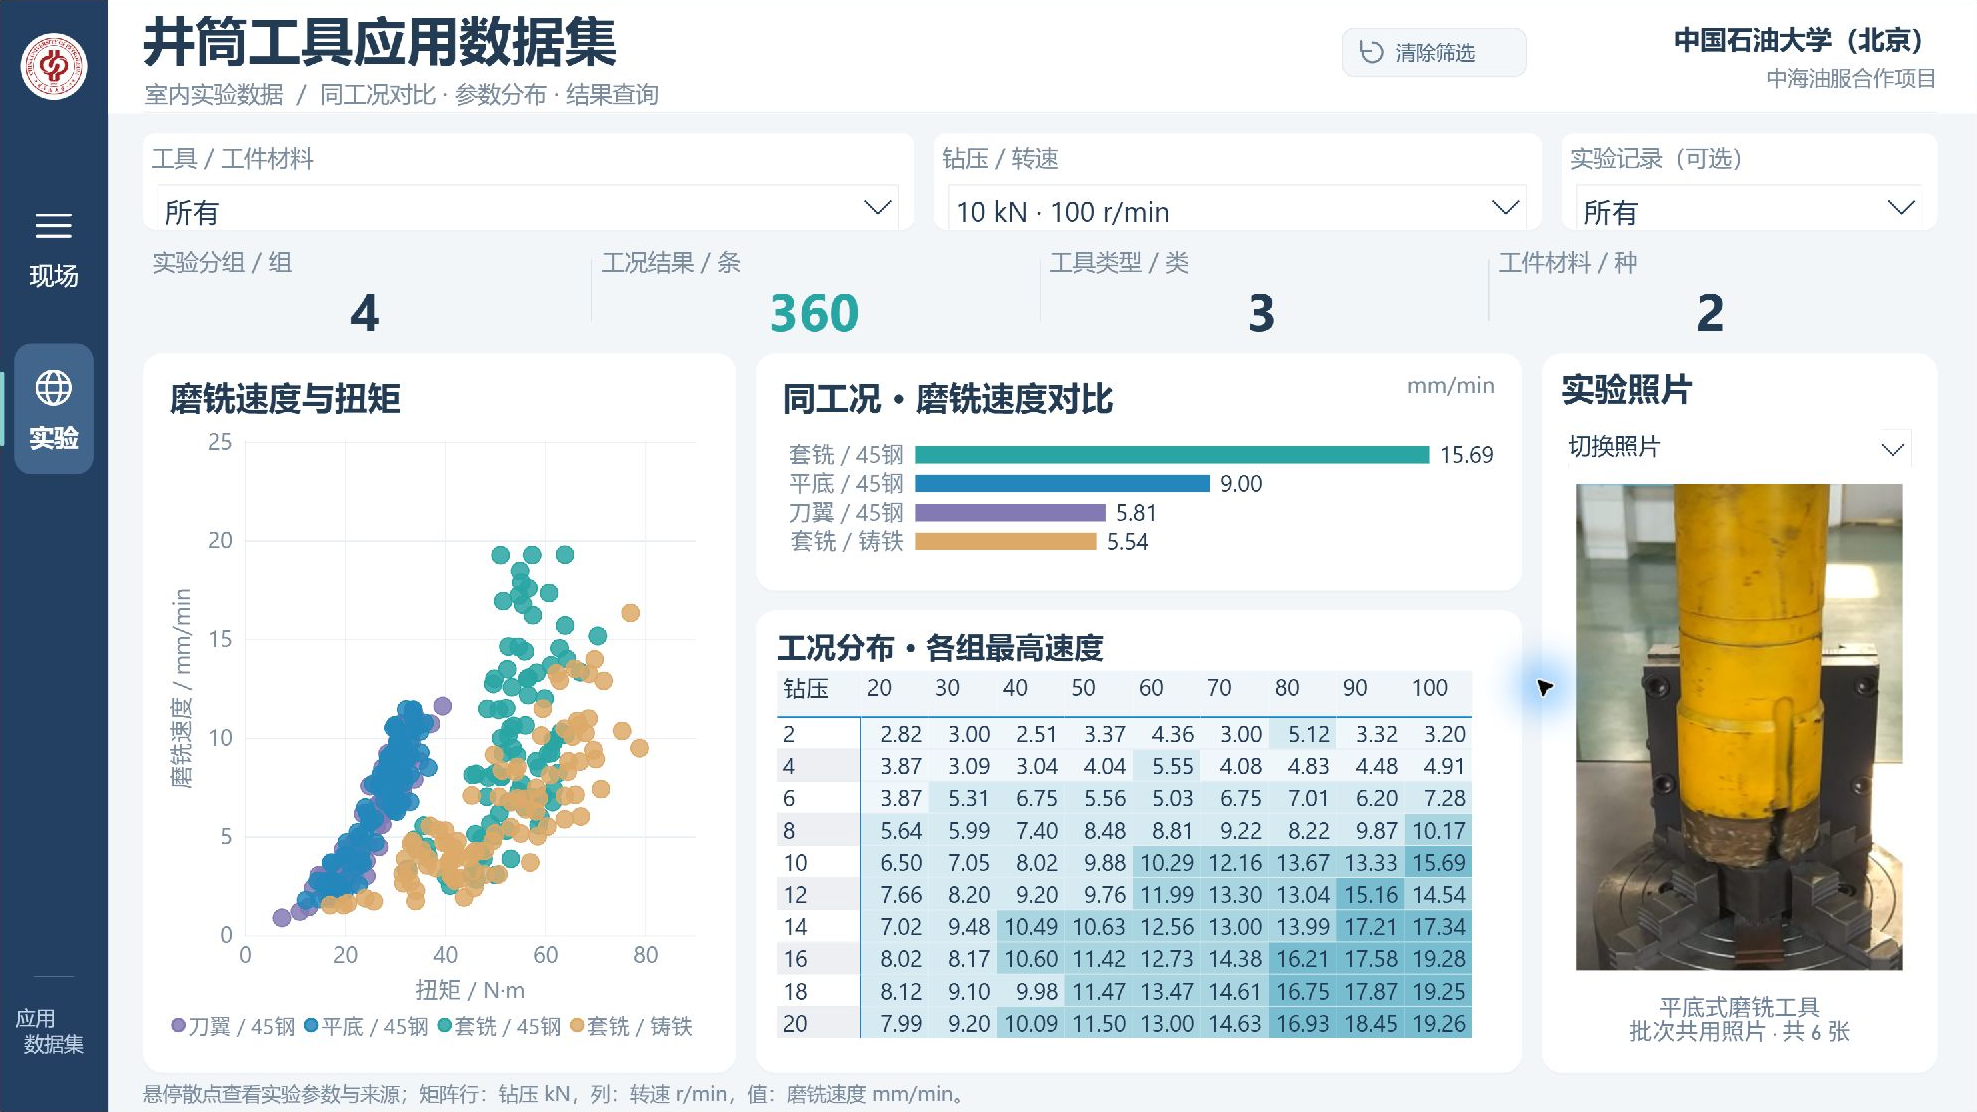
\includegraphics[width=120.000mm,height=0.76\textheight,keepaspectratio]{figure/research4-6/fig4-06-1.png}
\caption{井筒工具应用数据集室内实验查询界面}
\label{fig:r46-4-6}
\end{figure}

数据集配套现场及室内登记模板、照片关联规则、数据更新程序和使用手册。已形成8章逐步操作教程，覆盖资料整理、逐项填写、照片关联和刷新核对，支持新增记录进入同一查询工程。
